% Options for packages loaded elsewhere
% Options for packages loaded elsewhere
\PassOptionsToPackage{unicode}{hyperref}
\PassOptionsToPackage{hyphens}{url}
\PassOptionsToPackage{dvipsnames,svgnames,x11names}{xcolor}
%
\documentclass[
  letterpaper,
  DIV=11,
  numbers=noendperiod]{scrartcl}
\usepackage{xcolor}
\usepackage{amsmath,amssymb}
\setcounter{secnumdepth}{-\maxdimen} % remove section numbering
\usepackage{iftex}
\ifPDFTeX
  \usepackage[T1]{fontenc}
  \usepackage[utf8]{inputenc}
  \usepackage{textcomp} % provide euro and other symbols
\else % if luatex or xetex
  \usepackage{unicode-math} % this also loads fontspec
  \defaultfontfeatures{Scale=MatchLowercase}
  \defaultfontfeatures[\rmfamily]{Ligatures=TeX,Scale=1}
\fi
\usepackage{lmodern}
\ifPDFTeX\else
  % xetex/luatex font selection
\fi
% Use upquote if available, for straight quotes in verbatim environments
\IfFileExists{upquote.sty}{\usepackage{upquote}}{}
\IfFileExists{microtype.sty}{% use microtype if available
  \usepackage[]{microtype}
  \UseMicrotypeSet[protrusion]{basicmath} % disable protrusion for tt fonts
}{}
\makeatletter
\@ifundefined{KOMAClassName}{% if non-KOMA class
  \IfFileExists{parskip.sty}{%
    \usepackage{parskip}
  }{% else
    \setlength{\parindent}{0pt}
    \setlength{\parskip}{6pt plus 2pt minus 1pt}}
}{% if KOMA class
  \KOMAoptions{parskip=half}}
\makeatother
% Make \paragraph and \subparagraph free-standing
\makeatletter
\ifx\paragraph\undefined\else
  \let\oldparagraph\paragraph
  \renewcommand{\paragraph}{
    \@ifstar
      \xxxParagraphStar
      \xxxParagraphNoStar
  }
  \newcommand{\xxxParagraphStar}[1]{\oldparagraph*{#1}\mbox{}}
  \newcommand{\xxxParagraphNoStar}[1]{\oldparagraph{#1}\mbox{}}
\fi
\ifx\subparagraph\undefined\else
  \let\oldsubparagraph\subparagraph
  \renewcommand{\subparagraph}{
    \@ifstar
      \xxxSubParagraphStar
      \xxxSubParagraphNoStar
  }
  \newcommand{\xxxSubParagraphStar}[1]{\oldsubparagraph*{#1}\mbox{}}
  \newcommand{\xxxSubParagraphNoStar}[1]{\oldsubparagraph{#1}\mbox{}}
\fi
\makeatother

\usepackage{color}
\usepackage{fancyvrb}
\newcommand{\VerbBar}{|}
\newcommand{\VERB}{\Verb[commandchars=\\\{\}]}
\DefineVerbatimEnvironment{Highlighting}{Verbatim}{commandchars=\\\{\}}
% Add ',fontsize=\small' for more characters per line
\usepackage{framed}
\definecolor{shadecolor}{RGB}{241,243,245}
\newenvironment{Shaded}{\begin{snugshade}}{\end{snugshade}}
\newcommand{\AlertTok}[1]{\textcolor[rgb]{0.68,0.00,0.00}{#1}}
\newcommand{\AnnotationTok}[1]{\textcolor[rgb]{0.37,0.37,0.37}{#1}}
\newcommand{\AttributeTok}[1]{\textcolor[rgb]{0.40,0.45,0.13}{#1}}
\newcommand{\BaseNTok}[1]{\textcolor[rgb]{0.68,0.00,0.00}{#1}}
\newcommand{\BuiltInTok}[1]{\textcolor[rgb]{0.00,0.23,0.31}{#1}}
\newcommand{\CharTok}[1]{\textcolor[rgb]{0.13,0.47,0.30}{#1}}
\newcommand{\CommentTok}[1]{\textcolor[rgb]{0.37,0.37,0.37}{#1}}
\newcommand{\CommentVarTok}[1]{\textcolor[rgb]{0.37,0.37,0.37}{\textit{#1}}}
\newcommand{\ConstantTok}[1]{\textcolor[rgb]{0.56,0.35,0.01}{#1}}
\newcommand{\ControlFlowTok}[1]{\textcolor[rgb]{0.00,0.23,0.31}{\textbf{#1}}}
\newcommand{\DataTypeTok}[1]{\textcolor[rgb]{0.68,0.00,0.00}{#1}}
\newcommand{\DecValTok}[1]{\textcolor[rgb]{0.68,0.00,0.00}{#1}}
\newcommand{\DocumentationTok}[1]{\textcolor[rgb]{0.37,0.37,0.37}{\textit{#1}}}
\newcommand{\ErrorTok}[1]{\textcolor[rgb]{0.68,0.00,0.00}{#1}}
\newcommand{\ExtensionTok}[1]{\textcolor[rgb]{0.00,0.23,0.31}{#1}}
\newcommand{\FloatTok}[1]{\textcolor[rgb]{0.68,0.00,0.00}{#1}}
\newcommand{\FunctionTok}[1]{\textcolor[rgb]{0.28,0.35,0.67}{#1}}
\newcommand{\ImportTok}[1]{\textcolor[rgb]{0.00,0.46,0.62}{#1}}
\newcommand{\InformationTok}[1]{\textcolor[rgb]{0.37,0.37,0.37}{#1}}
\newcommand{\KeywordTok}[1]{\textcolor[rgb]{0.00,0.23,0.31}{\textbf{#1}}}
\newcommand{\NormalTok}[1]{\textcolor[rgb]{0.00,0.23,0.31}{#1}}
\newcommand{\OperatorTok}[1]{\textcolor[rgb]{0.37,0.37,0.37}{#1}}
\newcommand{\OtherTok}[1]{\textcolor[rgb]{0.00,0.23,0.31}{#1}}
\newcommand{\PreprocessorTok}[1]{\textcolor[rgb]{0.68,0.00,0.00}{#1}}
\newcommand{\RegionMarkerTok}[1]{\textcolor[rgb]{0.00,0.23,0.31}{#1}}
\newcommand{\SpecialCharTok}[1]{\textcolor[rgb]{0.37,0.37,0.37}{#1}}
\newcommand{\SpecialStringTok}[1]{\textcolor[rgb]{0.13,0.47,0.30}{#1}}
\newcommand{\StringTok}[1]{\textcolor[rgb]{0.13,0.47,0.30}{#1}}
\newcommand{\VariableTok}[1]{\textcolor[rgb]{0.07,0.07,0.07}{#1}}
\newcommand{\VerbatimStringTok}[1]{\textcolor[rgb]{0.13,0.47,0.30}{#1}}
\newcommand{\WarningTok}[1]{\textcolor[rgb]{0.37,0.37,0.37}{\textit{#1}}}

\usepackage{longtable,booktabs,array}
\usepackage{calc} % for calculating minipage widths
% Correct order of tables after \paragraph or \subparagraph
\usepackage{etoolbox}
\makeatletter
\patchcmd\longtable{\par}{\if@noskipsec\mbox{}\fi\par}{}{}
\makeatother
% Allow footnotes in longtable head/foot
\IfFileExists{footnotehyper.sty}{\usepackage{footnotehyper}}{\usepackage{footnote}}
\makesavenoteenv{longtable}
\usepackage{graphicx}
\makeatletter
\newsavebox\pandoc@box
\newcommand*\pandocbounded[1]{% scales image to fit in text height/width
  \sbox\pandoc@box{#1}%
  \Gscale@div\@tempa{\textheight}{\dimexpr\ht\pandoc@box+\dp\pandoc@box\relax}%
  \Gscale@div\@tempb{\linewidth}{\wd\pandoc@box}%
  \ifdim\@tempb\p@<\@tempa\p@\let\@tempa\@tempb\fi% select the smaller of both
  \ifdim\@tempa\p@<\p@\scalebox{\@tempa}{\usebox\pandoc@box}%
  \else\usebox{\pandoc@box}%
  \fi%
}
% Set default figure placement to htbp
\def\fps@figure{htbp}
\makeatother





\setlength{\emergencystretch}{3em} % prevent overfull lines

\providecommand{\tightlist}{%
  \setlength{\itemsep}{0pt}\setlength{\parskip}{0pt}}



 


\KOMAoption{captions}{tableheading}
\makeatletter
\@ifpackageloaded{caption}{}{\usepackage{caption}}
\AtBeginDocument{%
\ifdefined\contentsname
  \renewcommand*\contentsname{Table of contents}
\else
  \newcommand\contentsname{Table of contents}
\fi
\ifdefined\listfigurename
  \renewcommand*\listfigurename{List of Figures}
\else
  \newcommand\listfigurename{List of Figures}
\fi
\ifdefined\listtablename
  \renewcommand*\listtablename{List of Tables}
\else
  \newcommand\listtablename{List of Tables}
\fi
\ifdefined\figurename
  \renewcommand*\figurename{Figure}
\else
  \newcommand\figurename{Figure}
\fi
\ifdefined\tablename
  \renewcommand*\tablename{Table}
\else
  \newcommand\tablename{Table}
\fi
}
\@ifpackageloaded{float}{}{\usepackage{float}}
\floatstyle{ruled}
\@ifundefined{c@chapter}{\newfloat{codelisting}{h}{lop}}{\newfloat{codelisting}{h}{lop}[chapter]}
\floatname{codelisting}{Listing}
\newcommand*\listoflistings{\listof{codelisting}{List of Listings}}
\makeatother
\makeatletter
\makeatother
\makeatletter
\@ifpackageloaded{caption}{}{\usepackage{caption}}
\@ifpackageloaded{subcaption}{}{\usepackage{subcaption}}
\makeatother
\usepackage{bookmark}
\IfFileExists{xurl.sty}{\usepackage{xurl}}{} % add URL line breaks if available
\urlstyle{same}
\hypersetup{
  pdftitle={Lab 04 - old Binomial lab},
  pdfauthor={Insert your name here},
  colorlinks=true,
  linkcolor={blue},
  filecolor={Maroon},
  citecolor={Blue},
  urlcolor={Blue},
  pdfcreator={LaTeX via pandoc}}


\title{Lab 04 - old Binomial lab}
\usepackage{etoolbox}
\makeatletter
\providecommand{\subtitle}[1]{% add subtitle to \maketitle
  \apptocmd{\@title}{\par {\large #1 \par}}{}{}
}
\makeatother
\subtitle{STAT 5700}
\author{Insert your name here}
\date{Invalid Date}
\begin{document}
\maketitle


This lab will have you work with the Binomial distribution in R. We
begin with a tutorial to introduce the R commands associated with this
distributions. There is also a template exercise provided as an example
of how to format your answers neatly, integrating both math symbols and
R code. Task 1 is an odd-numbered exercise from the textbook, so you can
check your answers to help you verify \texttt{dbinom()} and
\texttt{pbinom()} work as you expect.

Let's begin by loading the necessary packages. Most of the functions in
this lab are in base R, meaning they don't require any additional
packages, but we'll load the \texttt{tidyverse} so we can use
\texttt{\%\textgreater{}\%} and \texttt{ggplot()} when doing some
additional exploration!

\begin{Shaded}
\begin{Highlighting}[]
\FunctionTok{library}\NormalTok{(tidyverse)}
\end{Highlighting}
\end{Shaded}

\section{Tutorial}\label{tutorial}

R includes many built in functions for common distributions. Commands
for each follow the same basic format. The abbreviated name of the
distribution is preceeded by once of four letters:

\begin{itemize}
\tightlist
\item
  ``d'' for the density function (probability distribution for discrete
  random variables)
\item
  ``p'' for the cumulative distribution function (cdf)
\item
  ``q'' for the quantile function (gives the x value for a given
  cumulative probability)
\item
  ``r'' for random (generates a random number based on the distribution)
\end{itemize}

The \textbf{binomial distribution} probability and cdf in R:

\begin{itemize}
\tightlist
\item
  \texttt{dbinom(x,\ size,\ prob)} -- returns \(p(x) = P(X = x),\)
  (probability distribution) values for a binomial random variable
  \(X\),
\item
  \texttt{pbinom(x,\ size,\ prob)} -- returns \(F(x) = P(X \leq x),\)
  values for the binomial distribution (cdf)
\end{itemize}

Note that both have three arguments defined as:

\begin{itemize}
\tightlist
\item
  \texttt{x} = the value of the random variable for which a probability
  is computed
\item
  \texttt{size} = number of trials (this is what we usually refer to as
  \(n\))
\item
  \texttt{prob} = probability of success on a trial (what we usually
  refer to as \(p\))
\end{itemize}

Note that \texttt{x} can be a vector, meaning you can compute multiple
probabilities with a single command!

\subsection{Binomial Example}\label{binomial-example}

Suppose \(X \sim b(10, 0.3)\). The probability that \(X = 2\) is given
by

\begin{Shaded}
\begin{Highlighting}[]
\FunctionTok{dbinom}\NormalTok{(}\DecValTok{2}\NormalTok{, }\DecValTok{10}\NormalTok{, }\FloatTok{0.3}\NormalTok{)}
\end{Highlighting}
\end{Shaded}

\begin{verbatim}
[1] 0.2334744
\end{verbatim}

The probability that \(X \leq 2\) is given by

\begin{Shaded}
\begin{Highlighting}[]
\FunctionTok{pbinom}\NormalTok{(}\DecValTok{2}\NormalTok{, }\DecValTok{10}\NormalTok{, }\FloatTok{0.3}\NormalTok{)}
\end{Highlighting}
\end{Shaded}

\begin{verbatim}
[1] 0.3827828
\end{verbatim}

Recall that \(P(X \leq 2) = P(X = 0) + P(X = 1) + P(X = 2)\), so we
could also have gotten the same result with the following code:

\begin{Shaded}
\begin{Highlighting}[]
\FunctionTok{dbinom}\NormalTok{(}\DecValTok{0}\NormalTok{, }\DecValTok{10}\NormalTok{, }\FloatTok{0.3}\NormalTok{) }\SpecialCharTok{+} \FunctionTok{dbinom}\NormalTok{(}\DecValTok{1}\NormalTok{, }\DecValTok{10}\NormalTok{, }\FloatTok{0.3}\NormalTok{) }\SpecialCharTok{+} \FunctionTok{dbinom}\NormalTok{(}\DecValTok{2}\NormalTok{, }\DecValTok{10}\NormalTok{, }\FloatTok{0.3}\NormalTok{)}
\end{Highlighting}
\end{Shaded}

\begin{verbatim}
[1] 0.3827828
\end{verbatim}

We could compute the probability for all possible values of
\(X = 0, 1, \dots , 10\) by making \texttt{x} a vector.

\begin{Shaded}
\begin{Highlighting}[]
\NormalTok{x }\OtherTok{\textless{}{-}} \FunctionTok{c}\NormalTok{(}\DecValTok{0}\SpecialCharTok{:}\DecValTok{10}\NormalTok{)}
\FunctionTok{dbinom}\NormalTok{(x, }\DecValTok{10}\NormalTok{, }\FloatTok{0.3}\NormalTok{)}
\end{Highlighting}
\end{Shaded}

\begin{verbatim}
 [1] 0.0282475249 0.1210608210 0.2334744405 0.2668279320 0.2001209490
 [6] 0.1029193452 0.0367569090 0.0090016920 0.0014467005 0.0001377810
[11] 0.0000059049
\end{verbatim}

We can do a sanity check to make sure that all of those densities sum to
1. That is, to verify \(\sum_S f(x) = 1\).

\begin{Shaded}
\begin{Highlighting}[]
\FunctionTok{sum}\NormalTok{(}\FunctionTok{dbinom}\NormalTok{(x, }\DecValTok{10}\NormalTok{, }\FloatTok{0.3}\NormalTok{))}
\end{Highlighting}
\end{Shaded}

\begin{verbatim}
[1] 1
\end{verbatim}

We can use the vector of densities to plot the pmf

\begin{Shaded}
\begin{Highlighting}[]
\NormalTok{data }\OtherTok{\textless{}{-}} \FunctionTok{data.frame}\NormalTok{(}\AttributeTok{x =}\NormalTok{ x,}
                   \AttributeTok{d =} \FunctionTok{dbinom}\NormalTok{(x, }\DecValTok{10}\NormalTok{, }\FloatTok{0.3}\NormalTok{))}

\FunctionTok{ggplot}\NormalTok{(}\AttributeTok{data =}\NormalTok{ data) }\SpecialCharTok{+}
  \FunctionTok{geom\_col}\NormalTok{(}\FunctionTok{aes}\NormalTok{(}\AttributeTok{x =}\NormalTok{ x, }\AttributeTok{y =}\NormalTok{ d))}
\end{Highlighting}
\end{Shaded}

\pandocbounded{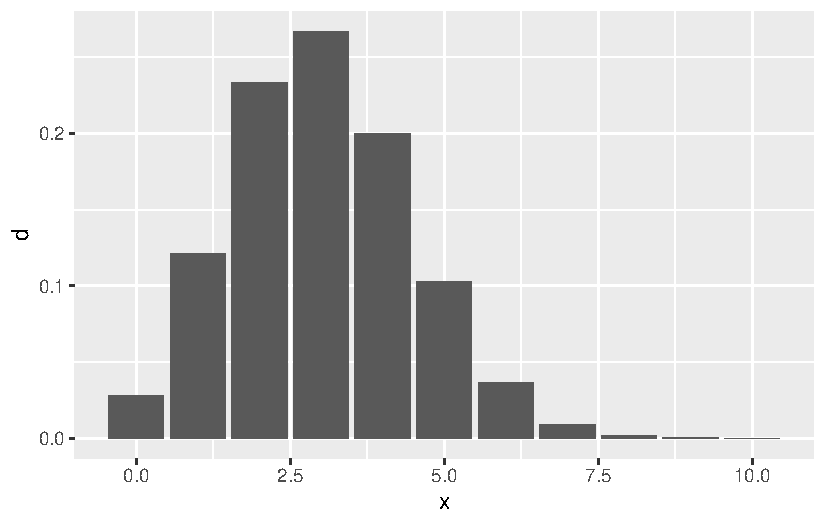
\includegraphics[keepaspectratio]{Lab_04-turn-into-in-class-handout_files/figure-pdf/unnamed-chunk-7-1.pdf}}

\begin{Shaded}
\begin{Highlighting}[]
\CommentTok{\# a prettier version of the plot}
\FunctionTok{ggplot}\NormalTok{(}\AttributeTok{data =}\NormalTok{ data) }\SpecialCharTok{+}
  \CommentTok{\#using factor(x) tells ggplot to treat x as discrete, }
  \CommentTok{\#so it labels the x axis at the integers 0:10}
  \CommentTok{\#fill = "skyblue" changes the color of the bars}
  \FunctionTok{geom\_col}\NormalTok{(}\FunctionTok{aes}\NormalTok{(}\AttributeTok{x =} \FunctionTok{factor}\NormalTok{(x), }\AttributeTok{y =}\NormalTok{ d), }\AttributeTok{fill =} \StringTok{"skyblue"}\NormalTok{) }\SpecialCharTok{+}
  \CommentTok{\#changes axis labels}
  \FunctionTok{labs}\NormalTok{(}\AttributeTok{x =} \StringTok{"x"}\NormalTok{, }\AttributeTok{y =} \StringTok{"Density f(x)"}\NormalTok{) }\SpecialCharTok{+}
  \FunctionTok{theme\_classic}\NormalTok{()}
\end{Highlighting}
\end{Shaded}

\pandocbounded{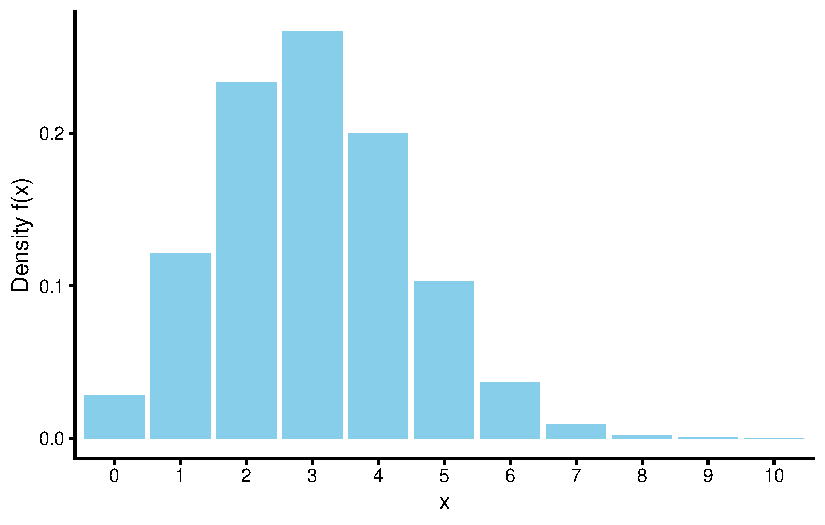
\includegraphics[keepaspectratio]{Lab_04-turn-into-in-class-handout_files/figure-pdf/unnamed-chunk-8-1.pdf}}

\subsection{Binomial mean \& variance}\label{binomial-mean-variance}

When working with the Binomial distribution, you can use the fact that
if \(Y \sim binom(n,p)\) then \(E(Y) = np\) and \(V(Y) = np(1-p)\) We
will prove this later on in the course.

\subsection{Template for Task
Solution}\label{template-for-task-solution}

\emph{You can use the following solution as a template for how to format
your solutions on Tasks 1 \& 2 below.}

A certain type of mint has a label weight of 20.4 grams. Suppose that
the probability is 0.90 that a mint weighs more than 20.7 grams. Let
\(X\) equal the number of mints that weigh more than 20.7 grams in a
sample of eight mints selected at random.

\begin{enumerate}
\def\labelenumi{\alph{enumi}.}
\tightlist
\item
  Find the mean and standard deviation of \(X\)
\item
  Find the probability that exactly 8 mints weigh more than 20.7 grams
\item
  Find the probability that no more that 6 mints weigh more than 20.7
  grams
\end{enumerate}

\subsection{ANSWER}\label{answer}

{[}OPTIONAL BUT ENCOURAGED: to help us verify that our answers are
reasonable, we can first plot the distribution{]}

\(X \sim b(8, 0.9)\)

\begin{Shaded}
\begin{Highlighting}[]
\CommentTok{\#create vector of possible x values}
\NormalTok{x }\OtherTok{\textless{}{-}} \FunctionTok{c}\NormalTok{(}\DecValTok{0}\SpecialCharTok{:}\DecValTok{8}\NormalTok{)}
\CommentTok{\#create vector of corresponding densities}
\NormalTok{d }\OtherTok{\textless{}{-}} \FunctionTok{dbinom}\NormalTok{(x, }\DecValTok{8}\NormalTok{, }\FloatTok{0.9}\NormalTok{)}
\CommentTok{\#combine into a data frame for plotting}
\NormalTok{data }\OtherTok{\textless{}{-}} \FunctionTok{data.frame}\NormalTok{(x, d)}

\FunctionTok{ggplot}\NormalTok{(}\AttributeTok{data =}\NormalTok{ data) }\SpecialCharTok{+}
  \FunctionTok{geom\_col}\NormalTok{(}\FunctionTok{aes}\NormalTok{(}\AttributeTok{x =} \FunctionTok{factor}\NormalTok{(x), }\AttributeTok{y =}\NormalTok{ d), }\AttributeTok{fill =} \StringTok{"navyblue"}\NormalTok{) }\SpecialCharTok{+}
  \FunctionTok{labs}\NormalTok{(}\AttributeTok{x =} \StringTok{"x"}\NormalTok{, }\AttributeTok{y =} \StringTok{"Density f(x)"}\NormalTok{) }\SpecialCharTok{+}
  \FunctionTok{theme\_classic}\NormalTok{()}
\end{Highlighting}
\end{Shaded}

\pandocbounded{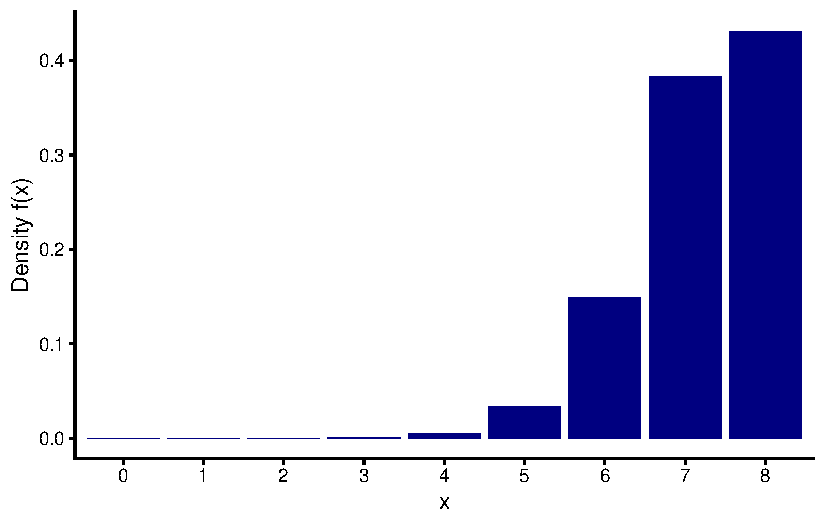
\includegraphics[keepaspectratio]{Lab_04-turn-into-in-class-handout_files/figure-pdf/unnamed-chunk-9-1.pdf}}

\subsubsection{Part a}\label{part-a}

\[\mu = np = 8 \cdot 0.9\]
\[\sigma = \sqrt{np(1-p)} = \sqrt{8 \cdot 0.9 \cdot 0.1}\]

\begin{Shaded}
\begin{Highlighting}[]
\NormalTok{mu }\OtherTok{\textless{}{-}} \DecValTok{8}\SpecialCharTok{*}\FloatTok{0.9}
\NormalTok{sigma }\OtherTok{\textless{}{-}} \FunctionTok{sqrt}\NormalTok{(}\DecValTok{8}\SpecialCharTok{*}\FloatTok{0.9}\SpecialCharTok{*}\FloatTok{0.1}\NormalTok{)}
\NormalTok{solution }\OtherTok{\textless{}{-}} \FunctionTok{data.frame}\NormalTok{(mu, sigma)}
\NormalTok{solution}
\end{Highlighting}
\end{Shaded}

\begin{verbatim}
   mu     sigma
1 7.2 0.8485281
\end{verbatim}

\subsubsection{Part b}\label{part-b}

\(P(X = 8)\)

\begin{Shaded}
\begin{Highlighting}[]
\FunctionTok{dbinom}\NormalTok{(}\DecValTok{8}\NormalTok{, }\AttributeTok{size =} \DecValTok{8}\NormalTok{, }\AttributeTok{prob =} \FloatTok{0.9}\NormalTok{)}
\end{Highlighting}
\end{Shaded}

\begin{verbatim}
[1] 0.4304672
\end{verbatim}

\subsubsection{Part c}\label{part-c}

\(P(X \leq 6)\)

\begin{Shaded}
\begin{Highlighting}[]
\FunctionTok{pbinom}\NormalTok{(}\DecValTok{6}\NormalTok{, }\AttributeTok{size =} \DecValTok{8}\NormalTok{, }\AttributeTok{prob =} \FloatTok{0.9}\NormalTok{)}
\end{Highlighting}
\end{Shaded}

\begin{verbatim}
[1] 0.1868953
\end{verbatim}

\section{Task 1}\label{task-1}

\emph{From Hogg, Tanis, and Zimmermann; Exercise 2.4-5}

In a lab experiment involving inorganic syntheses of molecular
precursors to organometallic ceramics, the final step of a five-step
reaction involves the formation of a metal--metal bond. The probability
of such a bond forming is \(p = 0.20\). Let \(X\) equal the number of
successful reactions out of \(n = 25\) such experiments.

\begin{enumerate}
\def\labelenumi{\alph{enumi}.}
\tightlist
\item
  Find the probability that \(X\) is at most 4.
\item
  Find the probability that \(X\) is at least 5.
\item
  Find the probability that \(X\) is equal to 6.
\item
  Give the mean, variance, and standard deviation of \(X\).
\end{enumerate}

\subsection{ANSWER}\label{answer-1}

\subsubsection{Part a}\label{part-a-1}

\subsubsection{Part b}\label{part-b-1}

\subsubsection{Part c}\label{part-c-1}

\subsubsection{Part d}\label{part-d}

\section{Task 2}\label{task-2}

It is believed that approximately 75\% of American youth now have
insurance due to the health care law. Suppose this is true, and let
\(X\) equal the number of American youth in a random sample of
\(n = 15\) with private health insurance.

\begin{enumerate}
\def\labelenumi{\alph{enumi}.}
\tightlist
\item
  Find the probability that \(X\) is at least 10.
\item
  Find the probability that \(X\) is at most 10.
\item
  Find the probability that \(X\) is equal to 10.
\item
  Give the mean, variance, and standard deviation of \(X\).
\end{enumerate}

\subsection{ANSWER}\label{answer-2}

\subsubsection{Part a}\label{part-a-2}

\subsubsection{Part b}\label{part-b-2}

\subsubsection{Part c}\label{part-c-2}

\subsubsection{Part d}\label{part-d-1}




\end{document}
